\newpage
\section{Hardware}
\begin{figure}[H]
	\centering
	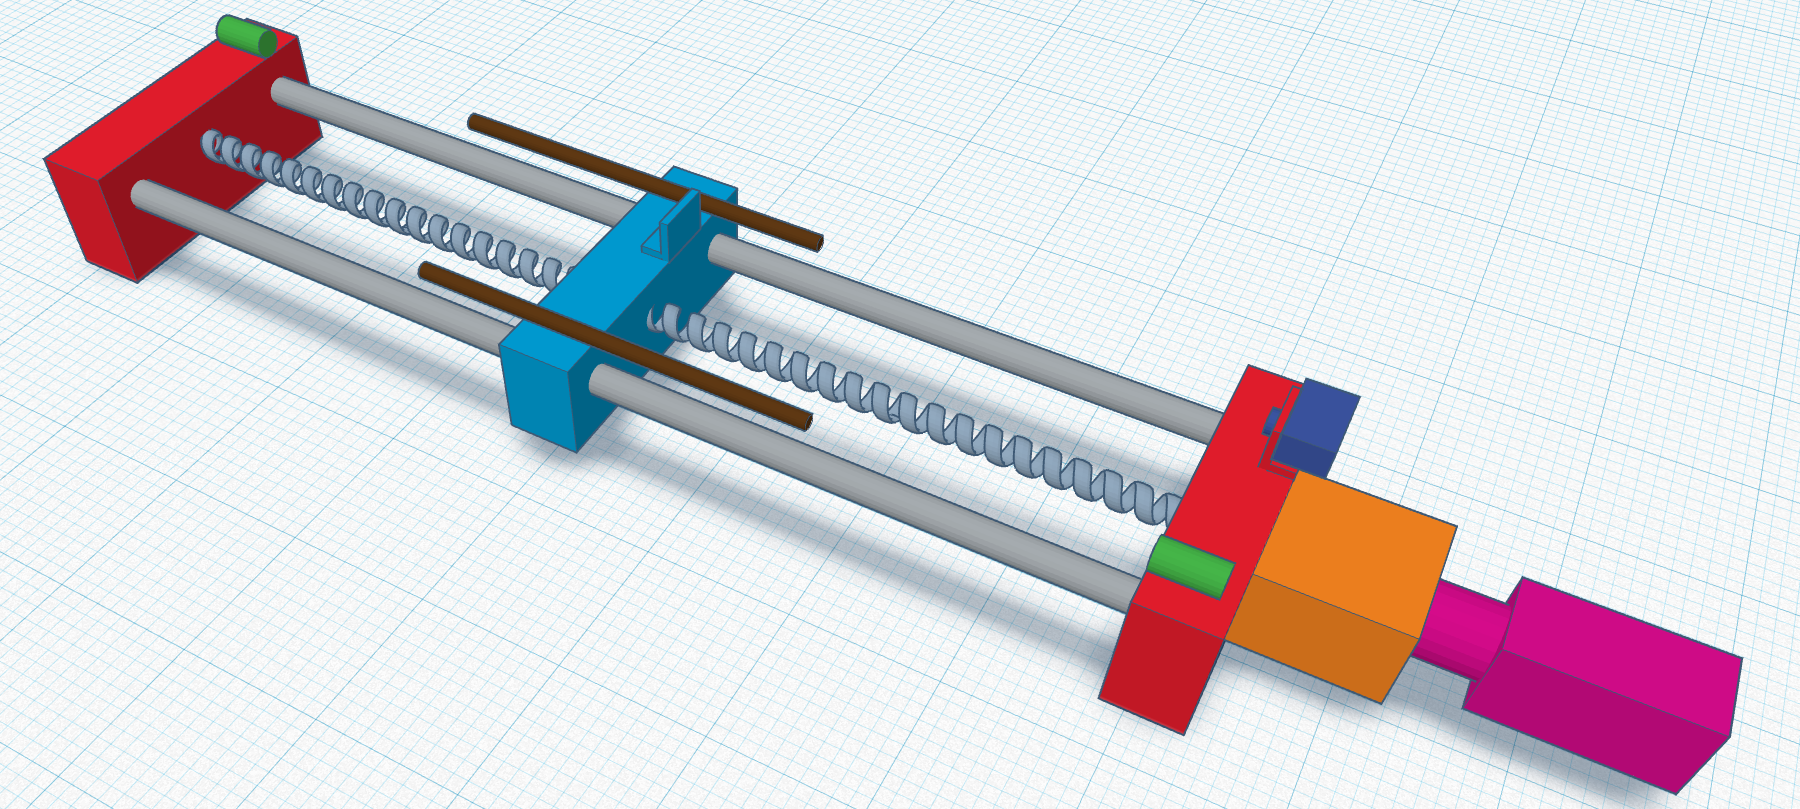
\includegraphics[width=1.0\textwidth]{images/Hardware/Linerarfuerhrung_3D_Modell.png}
	\caption{Simplifiziertes 3D Modell der Lineraführung}
	\label{fig:Systemaufbau}
\end{figure}
Da sich das Sailwind 4.0 Projekt noch in der Entwicklung befindet, existiert noch kein komplett zusammengebauter Prototyp in dem alle Teile des Projektes zusammenfinden. Die für diese Arbeit relevante Linearführung ist bereits als eigenständiges Objekt zusammengebaut und wie in \autoref{fig:Systemaufbau} zusehen, aufgebaut. Dabei wird die rotierende Bewegung eines BLDC Motors (Pink) mit der Hilfe eines Getriebes (Orange) und einer Gewindestange in eine translatorische Bewegung umgewandelt, mit welcher der Schlitten (Hellblau) zwischen den beiden stationären Punkten (Rot) hin und her bewegt werden kann. Die beiden Endschalter (Grün) dienen der Kollisionserkennung und können auch dazu genutzt werden, den Bewegungsraum einzuschränken. Dies gelingt durch das Verschieben der beiden Metallstangen (Braun), welche den Platz zwischen dem Schlitten und den stationären Elementen vorgeben. Zusätzlich kann über einen Abstandssensor (dunkel Blau) die Position des Schlittens in Relation zum Abstandssensor bestimmt werden.\\

\noindent Die Linearführung soll später dazu genutzt werden um die Segel des Windkraftwerkes zu trimmen und zu rollen (siehe Kapitel \ref{sec:principles}). Zusätzlich zu dem präsentierten Aufbau soll sich auf dem Schlitten zukünftig ein Druckkraftsensor befinden, der die Kraft auf die Rotorwelle messen soll. Dieser wurde allerdings zum Zeitpunkt der Arbeit noch nicht geliefert oder auf dem Prototypen angebracht. Getrennt vom Aufbau soll ebenfalls ein Anemometer an der Kuppel angebracht werden, das die Windrichtung und Geschwindigkeit misst.

%Hier erwähnen was Platine alles für Aufgaben hat
%Um die Segel des Windkraftwerkes jederzeit für maximale Effizienz eingestellt zu haben, müssen diese dynamisch Eingestellt werden können. Hierfür überwacht ein Controllino, die über Sensoren seine Umgebung und berechnet daraus die optimale Segel Einstellung. (KP sollte besser schon früher erwähnt werden/bzw wurde eventuell schon erwähnt)
\subsection{Ziele}
Die Hardware der Steuerung zu der eben vorgestellten Linearführung soll dabei folgende Aufgaben übernehemen:
\begin{itemize}
	\item Ansteuerung aller Sensoren und Aktoren
	\item Stromversorgung aller Komponenten
	\item Lokale Bedienung der Steuerung
	\item Ethernetkommunikation mit dem Controllino
\end{itemize}

\noindent Neben diesen Aufgaben soll die ganze Steuerung in einem zumindest Staub- und Spritzwassergeschützten Gehäuse untergebracht werden. Die Vorgängergruppe hatte sich dieser Aufgabe bereits gewidmet, allerdings wurde der resultierende Prototyp aufgrund der aufgetretenen Fehler und des zu großen Formfaktors nicht weiter verwendet. Diese Probleme sollen in dieser Iteration ebenfalls behoben werden.

%Bei dem Entwurf der Hardware sind mehrere Dinge zu beachten. Da das Sailwind 4.0 Projekt noch in den Startschuhen steht, sind einige dieser Faktoren auch noch nicht klar Bestimmbar zum Zeitpunkt dieser Arbeit. Aus diesem Grund wurden an manchen Stellen die Design Kriterien freier oder unnötig Komplex ausgelegt.\\
%
%Um die Steuerung der Segel zu ermöglichen wird ein System benötigt das alle nötigen Akteure und Sensoren, Ansteuret und Überwacht. Hierfür soll eine Steuerelektronik Hardware entworfen werden. Da sich diese im Außeneinsatz befindet sollte diese in einem Wasserdichten Gehäuse eingeschlossen sein. Eine vorrausgehende Gruppe hatte bereits die Steuerelektronik entworfen, diese war allerdings zu groß dimensioniert und hatte einige Fehler, weswegen ebenfalls ein kleinere Formfaktor und die Behebung der Probleme als Ziel gesetzt wurden. Die Steuerelektronik soll Manuell Bedienbar sein, wewegen am Gehäuse ebenfalls eine Bedienmöglichkeit existieren sollte.

\label{Analyze_der_Aktoren_und_Sensoren}
\subsection{Analyse der bestehenden Hardware Elemente}
Um eine geeignete Steuerplatine zu entwerfen, bedarf es einer Analyse der Steuerelemente, welche bereits von der vorhergegangenen Gruppe festgelegt wurden. Diese können in die Kategorien Sensoren und Aktoren gruppiert werden. Dabei wurden die benötigte Spannung und die Schnittstellen betrachtet. Die Schnittstellen geben an, wie mit dem jeweiligen Gerät kommuniziert werden kann und welche davon benötigt werden. Über die Spannung kann die Versorgungsspannung der Platine ausgewält werden und bereits ein Spannungspotenzial festgelegt werden.\\

\subsubsection{Sensoren}
Zu den Sensoren zählen die folgenden Komponenten:
\begin{itemize}
	\item Induktiver Endschalter: IFM IFS204
	\item Optischer Abstandssensor: IFM OGD580
	\item Anemometer: MESA WSWD
	\item Druckkraft-Sensor: Burster 8532
\end{itemize}

\noindent\textbf{Induktiver Endschalter}\newline
Zwei der IFM IFS204 Endschalter sind im Design mit eingebaut. Sie funktionieren als PNP-Schließkontakt und geben an einem Ausgang ein digitales 24V Signal aus, sobald sie ausgelöst werden. Dabei hat jeder Endschalter eine Betriebsspannung von 9-30V.\\

\noindent\textbf{Optischer Abstandssensor}\newline
Der Abstandssensor OGD580 funktioniert über einen Laser der vom Gerät ausgehend über eine Reflektive Fläche zu diesem zurückgeworfen wird. Der Abstandsensor verfügt über ein Display das den gemessenen Abstand anzeigt und über das Gerät konfigurierbar ist. Er hat ebenfalls eine Betriebspannung von 9-30V. Der Abstand wird über einen digitalen Ausgang, dem sog. IO-Link ausgegeben. Da mit diesem nur sehr umständlich Umgegange werden kann, wurde ein zusätzlicher IO-Link Konverter hinzugefügt. Der EIO104 konvertiert die digitale IO-Link Schnittstelle zu einer analogen 4-20mA Schnittstelle mit der einfacher Umgegangen werden kann.\\

\noindent\textbf{Anemometer}\\
Das WSWD Anemometer wird genutzt, um die Windrichtung und -geschwindigkeit zu messen. Dieses basiert auf einer 24V Versorgungsspannung. Es besitzt ebenfalls ein Heizelement, das die Verwendung bei sehr niedrigen Temperaturen ermöglicht. Dieses wird allerdings im Einsatzszenario und im Prototyp nicht benötigt. Die Schnittstellen des Anenometers sind abhängig von dessen Ausführung. In der verwendeten Ausführung, dem WSWD1, können die Daten neben einer analogen auch über eine Digitale RS485/RS422 Schnittstelle abgefragt werden. Die Werte können Analog entweder als 0/4-20/24mA Strom- oder als 0/2-8/10V Spannungssignal ausgegeben werden. Die Digitale Schnittstelle kann neben der Datenausgabe auch zur Konfiguration des Gerätes genutzt werden und bietet eine Vielzahl an Konfigurationsparametern und Übertragungsprotokollen an.\\

\noindent\textbf{Druckkraft-Sensor}\newline
Der Burster Druckkraft-Sensor war der einzige Sensor der zum Zeitpunkt der Arbeit noch nicht im Prototyp mit eingebaut wurde. Dieser wurde aber dennoch mit eingeplant. Der Druckkraft Sensor kann ebenfalls mit den typischen 24V betrieben werden. Die Messwerte werden hier über eine Analoges 0-10V Spannungssignal übertragen.\\

\noindent\textbf{Temperatursensor}\newline
Ähnlich zu den Relais gibt es noch keine genaueren Informationen zu einem eventuell zum Einsatz kommenden Temperatursensor. Es wurde dennoch ein zusätzlicher analoger Eingang für eine entsprechende 4-20mA Schnittstelle eingeplant.\\
\subsubsection{Aktoren}
Zu den Aktoren zählen die folgenden Komponenten:
\begin{itemize}
	\item Gleichstrommotor: Dunkermotoren BG 45x30 SI
	\item Externe Relais
\end{itemize}

\noindent\textbf{Gleichstrommotor}\newline
Der Dunker BG 45x30 SI Gleichstrommotor ist die antreibende Kraft im Aufbau. Da der Motor eine interne Regelung besitzt, sind Leistungs- und Logikversorgung getrennt. Der Motor an sich wird dabei über den Leistungsteil bestromt, während der Logikteil für die Steuerung und die Bereitstellung von Feedback-Daten zuständig ist. Die Betriebsspannung der Leistungs- und Logikversorgung liegt bei 24V, wobei der Leistungsteil einem maximal zulässigen Dauerstrom von 3,8A ausgesetzt sein darf. Die Ansteuerung des Motors findet über vier digitale- und einen analogen Eingang statt. Der Motor stellt Feedback zum aktuellen Status über drei Ausgänge bereit. Diese geben die Drehrichtung, aktuelle Störungen und die Drehgeschwindigkeit des Motors in Impulsen an. Die Bezeichnung und Funktionen dieser Ein-/Ausgänge sind in \autoref{tab:digitale_Eingaenge}/\autoref{tab:andere_Ausgaenge} dargestellt.\\
% Please add the following required packages to your document preamble:
% \usepackage{graphicx}
\begin{table}[H]
	\centering
		\begin{tabular}{|c|c|c|}
			\hline
			\textbf{Eingang 1 (IN1)} & \textbf{Eingang 0 (IN0)} & \textbf{Funktion}      \\ \hline
			0                        & 0                        & Motor aus              \\ \hline
			0                        & 1                        & Linkslauf              \\ \hline
			1                        & 0                        & Rechtslauf             \\ \hline
			1                        & 1                        & Stopp mit Haltemoment  \\ \hline
			\textbf{Eingang 3 (IN3)} & \textbf{Eingang 2 (IN2)} &                        \\ \hline
			0                        & 0                        & Drehzahlvorgabe Analog \\ \hline
			0                        & 1                        & Stromvorgabe Analog    \\ \hline
			1                        & 0                        & Geschwindigkeit 1      \\ \hline
			1                        & 1                        & Geschwindigkeit 2      \\ \hline
		\end{tabular}%
	\caption{Eingänge und Funktionen des BG 45x30 SI}
	\label{tab:digitale_Eingaenge}
\end{table}
\begin{table}[H]
	\centering
	\begin{tabular}{|c|c|c|}
		\hline
		\textbf{Name} & \textbf{Wertebereich} & \textbf{Funktion}      \\ \hline
		Analog In                & 0-4092$\frac{U}{min}$                        & Drehzahlvorgabe/            \\ & 0-10V & Analogwert \\ \hline		Out 1                & 12$\frac{Impulse}{U}$                        & Aktuelle Drehzahl             \\ \hline
		Out 2                & 1 = Störung; 0 = keine Störung                        &  Fehlerangabe            \\ \hline
		Out 3              & 1 = Linkslauf; 0 = Rechtslauf                       &  Drehrichtung           \\ \hline
	\end{tabular}%
	\caption{Analoger Eingang und Digitale Ausgänge des BG 45x30 SI}
	\label{tab:andere_Ausgaenge}
\end{table}

\noindent\textbf{Externe Relais}\newline
Zum Zeitpunkt der Arbeit gab es noch keinen konkreten Verwendungszweck der zwei externen Relais, diese wurden für zusätzliche Funktionalitäten dennoch mit eingeplant und sollten über ein 24V Signal geschaltet werden. Sie könnten z.B zum Auslösen einer Motorbremse genutzt werden.\\

\noindent\textbf{Controllino}\newline
Der Controllino ist der zentrale Microcontroller und verwaltet alle Aktoren im fertigen Sailwind 4.0 Prototyp. Von diesem soll das in der Arbeit zu entwerfende System seine Befehle zur Segelausrichtung empfangen. Der Datenaustausch soll dabei über Ethernet stattfinden, um die große Distanz zwischen Kuppel und Basis des Kraftwerkes zu überbrücken. Zusätzlich ist geplant die Platine vom Controllino mit Strom zu versorgen.
\subsubsection{Zusammenfassung und Übersicht}
Damit sind nun alle externen Komponente im System abgedeckt. Die benötigte Spannungsversorgung sowie alle Schnittstellen sind in \autoref{tab:uebersicht-externe-elemente} dargestellt. Zusätzlich wurden die Verbindungen in einem Blockschaltbild in \autoref{fig:System_Aufbau} zusammengefasst, wobei alle blauen Pfeile die digitalen 24V Ein- und Ausgänge beschreiben.
\begin{figure}[H]
	\centering
	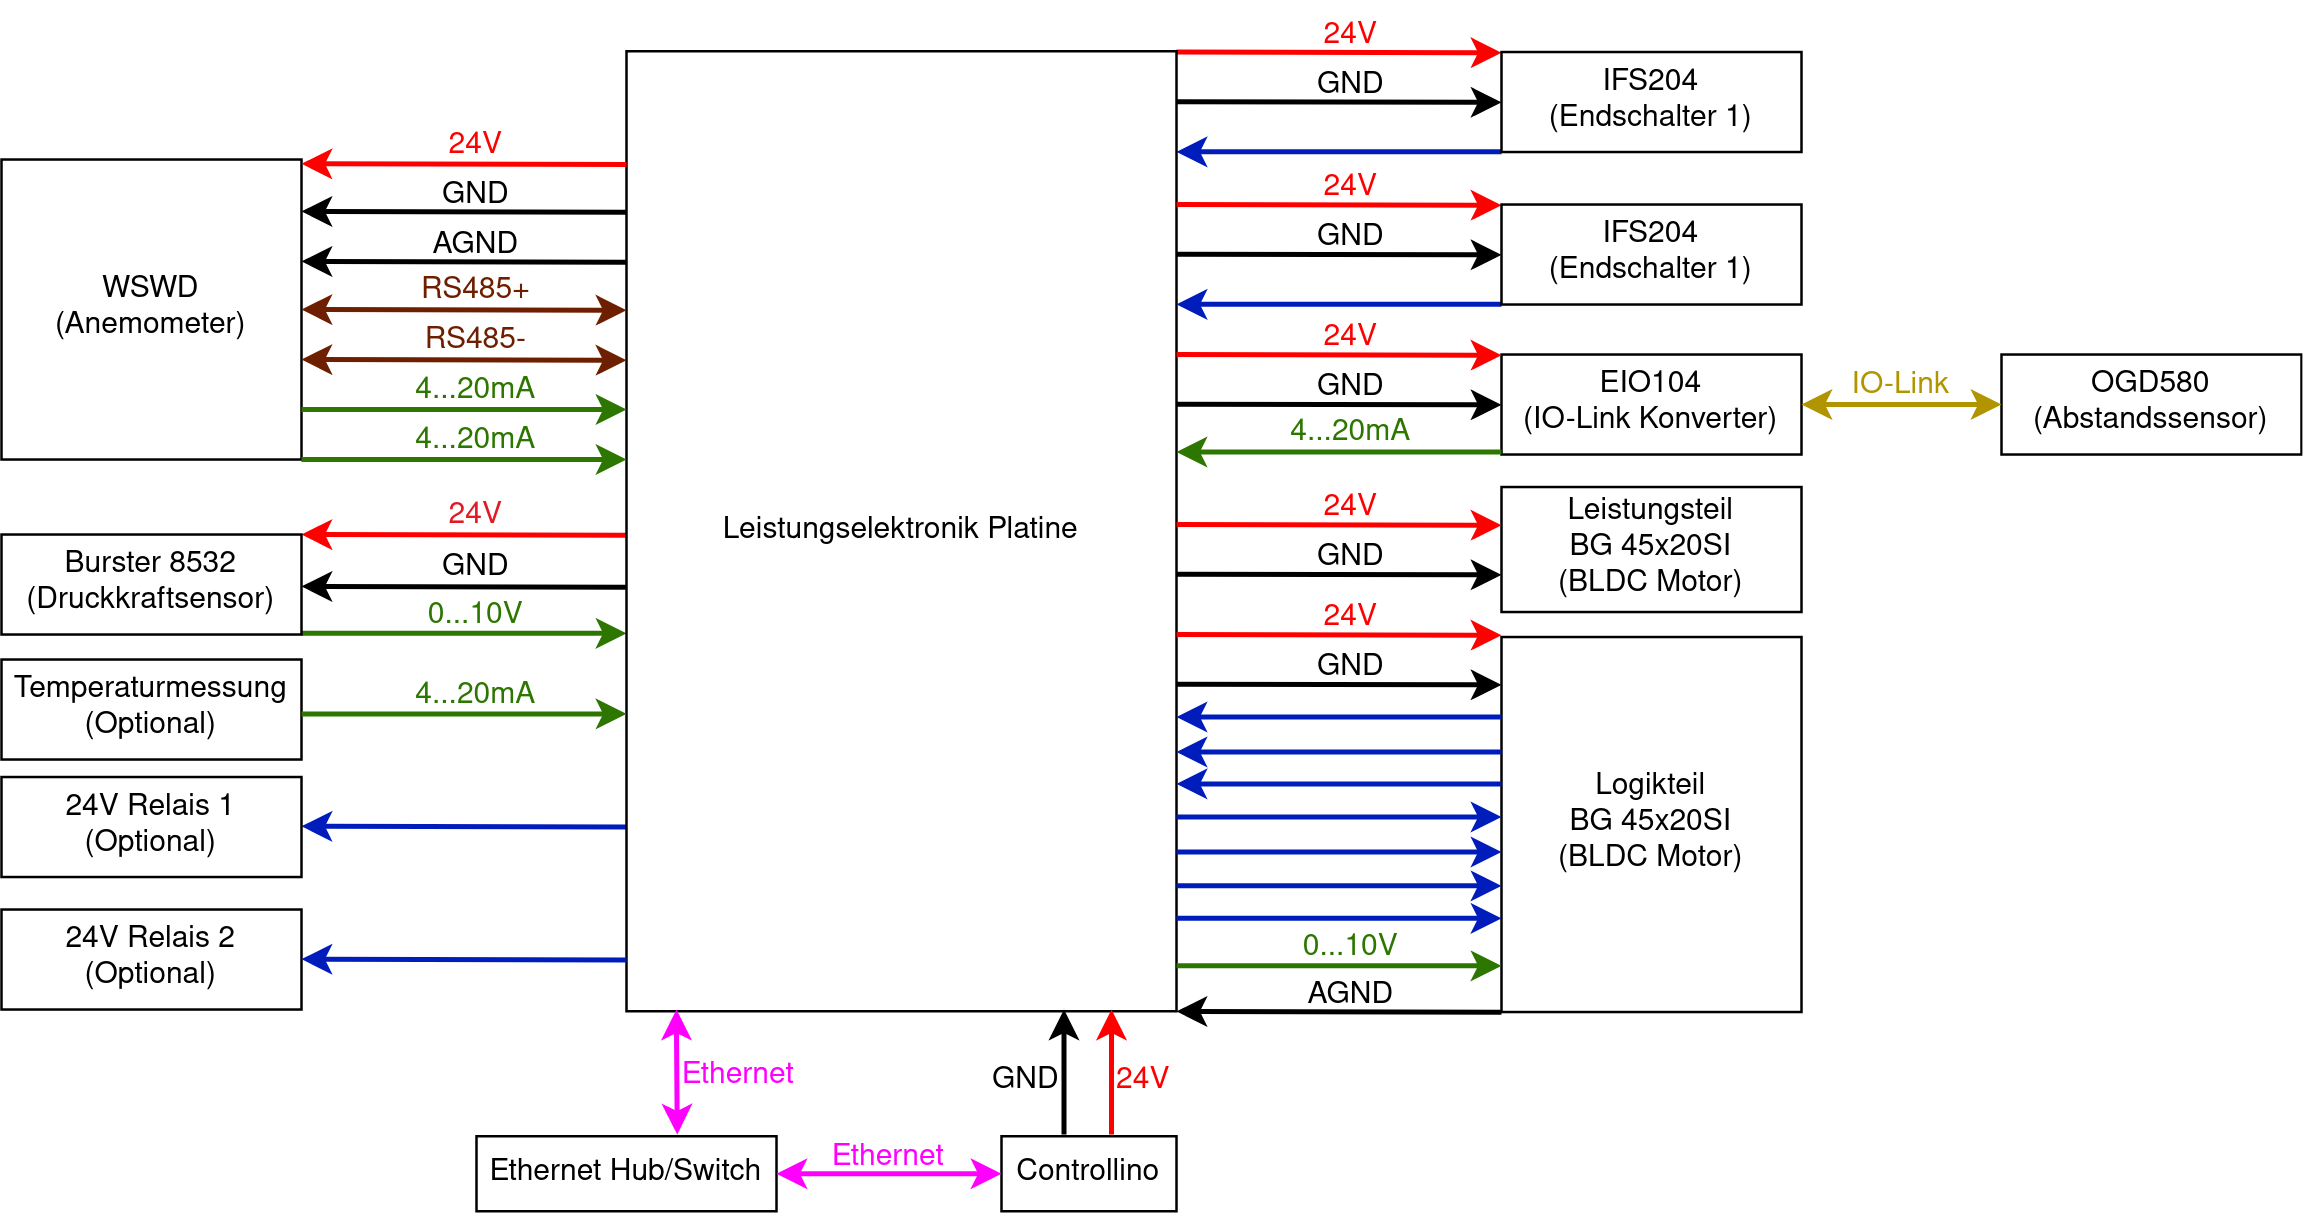
\includegraphics[width=1.0\textwidth]{images/System/Systemaufbau.drawio.png}
	\caption{Blockschaltbild der benötigten Ein- und Ausgänge der Platine}
	\label{fig:System_Aufbau}
\end{figure}
% Please add the following required packages to your document preamble:
% \usepackage{graphicx}
\begin{table}[H]
	\centering
	\resizebox{\textwidth}{!}{%
		\begin{tabular}{|l|lllllllllll|}
			\hline
			\textbf{Element} & \multicolumn{11}{l|}{\textbf{Pinout}} \\ \hline
			\textbf{Endschalter 1} & \multicolumn{1}{l|}{24V} & \multicolumn{1}{l|}{GND} & \multicolumn{1}{l|}{OUT} & \multicolumn{8}{l|}{} \\ \hline
			\textbf{Endschalter 2} & \multicolumn{1}{l|}{24V} & \multicolumn{1}{l|}{GND} & \multicolumn{1}{l|}{OUT} & \multicolumn{8}{l|}{} \\ \hline
			\textbf{Abstandssensor} & \multicolumn{1}{l|}{24V} & \multicolumn{1}{l|}{GND} & \multicolumn{1}{l|}{IO-Link} & \multicolumn{8}{l|}{} \\ \hline
			\textbf{IO-Link Konveter} & \multicolumn{1}{l|}{24V} & \multicolumn{1}{l|}{GND} & \multicolumn{1}{l|}{AOUT} & \multicolumn{8}{l|}{} \\ \hline
			\textbf{Anemometer} & \multicolumn{1}{l|}{24V} & \multicolumn{1}{l|}{GND} & \multicolumn{1}{l|}{AOUT} & \multicolumn{1}{l|}{AOUT} & \multicolumn{1}{l|}{AGND} & \multicolumn{1}{l|}{RS485+} & \multicolumn{1}{l|}{RS485-} & \multicolumn{4}{l|}{} \\ \hline
			\textbf{Druckkraftsensor} & \multicolumn{1}{l|}{24V} & \multicolumn{1}{l|}{GND} & \multicolumn{1}{l|}{AOUT} & \multicolumn{1}{l|}{AGND} & \multicolumn{7}{l|}{} \\ \hline
			\textbf{Motor Leistung} & \multicolumn{1}{l|}{24V} & \multicolumn{1}{l|}{GND} & \multicolumn{9}{l|}{} \\ \hline
			\textbf{Motor Logik} & \multicolumn{1}{l|}{24V} & \multicolumn{1}{l|}{GND} & \multicolumn{1}{l|}{IN0} & \multicolumn{1}{l|}{IN1} & \multicolumn{1}{l|}{IN2} & \multicolumn{1}{l|}{IN3} & \multicolumn{1}{l|}{AIN} & \multicolumn{1}{l|}{AGND} & \multicolumn{1}{l|}{OUT1} & \multicolumn{1}{l|}{OUT2} & OUT3 \\ \hline
			\textbf{Externes Relais 1} & \multicolumn{1}{l|}{OUT} & \multicolumn{1}{l|}{GND} & \multicolumn{9}{l|}{} \\ \hline
			\textbf{Externes Relais 2} & \multicolumn{1}{l|}{OUT} & \multicolumn{1}{l|}{GND} & \multicolumn{9}{l|}{} \\
			\hline
			\textbf{Temperatur Sensor} & \multicolumn{1}{l|}{AOUT} & \multicolumn{10}{l|}{} \\ \hline
			\textbf{Controllino} & \multicolumn{1}{l|}{Ethernet} & \multicolumn{10}{l|}{} \\ \hline
		\end{tabular}%
	}
	\caption{Übersicht Stromversorgung und Schnittstellen der externen Elemente}
	\label{tab:uebersicht-externe-elemente}
\end{table}
\subsection{Auswahl der Platinen Bauteile}
Da nun klar ist, welche Anforderungen durch die anzuschließenden Geräte bestehen, kann auf Basis dieser weiter verfahren werden. Dabei soll im folgenden ein geeigneter Mikrocontroller, sowie die nötigen Platinenkomponenten ausgewählt werden, um mit den Sensoren und Aktoren zu kommunizieren und diese mit Strom zu versorgen.
\subsubsection{Mikrocontroller}
Die Auswahl des Mikrocontrollers wurde auf der Basis folgender Kriterien beschlossen:
\begin{itemize}
	\item Benötigte Inputs und Outputs
	\item Softwaresupport 
	\item Entwicklung
	\item Verfügbarkeit
\end{itemize}
Dabei gab es die Option, den Chip als einzelnes Element direkt in der selbst erstellten Platine einzubetten oder ein Entwicklungsboard zusammen mit einer Erweiterungsplatine zu nutzen. Schließlich fiel die Entscheidung auf die Verwendung eines Entwicklungsboards, um bereits parallel zum Hardwaredesign eine geeignete Software entwickeln und mit prototypischen Aufbauten testen zu können. Dies bot ebenfalls den Vorteil, dass ein kaputter Chip schnell ersetzt werden kann und mit der Platine ein möglicher Formfaktor für die Erweiterung vorgegeben ist. Außerdem kann durch den integrierten Debugger schneller neue Software getestet und aufgespielt werden. Zuletzt besitzen viele Entwicklungsboards bereits einen Ethernet-Port, der somit nicht mehr extra bestellt werden müsste.\\

\noindent Aufgrund der oben genannten Kriterien und der Entscheidung, ein Entwicklungsboard zu benutzen viel die Wahl auf das STM32 NUCLEO F439zi Board. Dieses war bereits an der HTWG Konstanz verfügbar und ist mit dem Softwaresupport der Firma ST, welche insbesondere eine eigene Entwicklungsumgebung anbietet, einfach zu programmieren und aufzusetzen. Außerdem enthalten Entwicklungsboards von ST einen abbrechbaren Debugger, womit das Board auch außerhalb der Entwicklungsphase eingesetzt werden kann.
\subsubsection{Relais}
Um das Auslösen eines Endschalters an den Mikrocontroller weiterzugeben, werden zwei 24V Relais benötigt, die bei Aktivierung der Spule ein 3,3V Signal an den Eingang des Mikrocontrollers weitergeben. Gleichzeitig soll durch die Relais der Eingang 1 oder 2 des Motors auf Null gesetzt werden. Diese geben die Drehrichtung vor und stoppen den Motor, sobald beide auf null gesetzt sind. Da dieses System unabhängig von der Software des Mikrocontrollers agiert, bietet es eine zusätzliche Sicherheit gegenüber Beschädigungen an der Linearführung aufgrund von Programm-Fehlfunktionen. Hierfür wurden die Omron G6S-2F 24DC Relais ausgewählt. Diese besitzen zwei schaltbare Ausgänge und weisen einen kompakten Formfaktor auf.
\subsubsection{Optokoppler}
Um die restlichen 24V Ein- und Ausgänge zu steuern oder auszulesen, kommen Optokoppler zum Einsatz. Diese isolieren ähnlich zu Relais den 24V und 3,3V Schaltkreis. Davon werden insgesamt neun benötigt, um die digitalen Ein- und Ausgänge des Motors und die beiden externen Relais zu schalten. Zusätzlich sollte wie bei den Relais wieder ein kleiner Formfaktor vorliegen. Hierfür wurden die LTV-817S ausgesucht. Deren typische Schaltzeit von 3-18$\mu$s ist für die Anwendung ausreichend und durch den Formfaktor lassen sich die Optokoppler gut auf der Platine unterbringen.
\subsubsection{RS485 zu UART Konverter}
Um das Anemometer über die RS485 Schnittstelle zu konfigurieren und Daten abzufragen wird ein zusätzlicher Baustein benötigt. Dieser konvertiert das differenzielle RS485-Signal zu einem nicht differenziellen \ac{UART}-Signal, welches der Mikrocontroller verarbeiten kann. Hierfür wurde der MAX3485CSA+CT-ND ausgesucht, da dieser mit einer 3,3V Versorgungsspannung betrieben werden kann und eine Datenübertragungsrate von bis zu 10$\frac{MB}{s}$ unterstützt.
\subsubsection{FRAM}
Da die neutrale Position des Segels dauerhaft gespeichert werden soll, wird ein nicht flüchtiger Speicherstein benötigt. Dabei ist \ac{FRAM} eine der billigsten Speichermöglichkeiten für diesen Zweck. Es wurde die geringste Speichergröße gewählt, da die gespeicherten Daten jederzeit, wie bei einem EEPROM Speicher, überschrieben werden können. Hier wurde der FM25L16B-GTR gewählt, welcher mit einer Speicherkapazität von 16Kbit ausgestattet ist und damit für das Speichern der Positionsdaten geeignet ist. Da er über eine \ac{SPI} Schnittstelle angesteuert wird, sind schnelle Schreib- und Lesegeschwindigkeiten möglich, was für das regelmäßige Aktualisieren der Positionsdaten erforderlich ist. Ebenfalls ist die Lebenserwartung des Speichers von 85 Jahren unter Betrieb mit einer Taktfrequenz von 20Mhz mehr als ausreichend.
\subsubsection{Operations Verstärker}
Um die Drehzahl des Motors vorgeben zu können, wird ein analoges Signal im Bereich von 0-10V benötigt. Da der \ac{DAC} des Mikrocontrollers bei einer Versorgungsspannung von 5V maximal ein analoges Signal von 3,3V ausgeben kann \cite{STM32}, wird ein Operationsverstärker benötigt. Dieser soll mit einer 24V Offsetspannung das Ausgangssignal auf 10V skalieren. Hier gab es bis auf die Maximalspannung keine besonderen Anforderungen an den Operationsverstärker und somit wurde der weitverbreitete LM2904QS ausgewählt.
\subsubsection{DC/DC-Wandler}
Um alle Komponenten zu versorgen, bedarf es insgesamt drei verschiedenen Spannungspotenzialen: 24V, 5V und 3,3V. Dabei werden alle externen Steuerelemente direkt mit 24V versorgt. Der Mikrocontroller benötigt eine 5V Spannung, damit dieser auch ohne Stromversorgung des Debuggers betrieben werden kann. Hierfür wird ein Step-Down Konverter genutzt, der die 24V Versorgungsspannung auf 5V herunterbricht. Die 5V müssen zusätzlich mit einem Festspannungsregler auf 3,3V-Level konvertiert werden, um die übrigen Bauteile zu versorgen. Bei der Auswahl wurde darauf geachtet, dass der Konverter einen ausreichenden Strom zu Verfügung stellt, ohne dabei dauerhaft unter Vollast zu laufen. Insbesondere muss hier der Verbrauch des Mikrocontrollers von bis zu 120mA (vgl. \cite{STM32_Electrical} S.103) eingerechnet werden. Unter der Annahme, dass die restlichen Bauteile nicht mehr als zusätzliche 380mA verbrauchen, wurde der R-78E5.0-0.5 ausgewählt. Dieser stellt bis zu 0,5A zur Verfügung und kann bei Bedarf durch eine 1A Version ausgetauscht werden. Als Festspannungsregler wurde der LM3940IMP-3.3 gewählt. Dieser kann Eingangsspannung von bis zu 7.5V in eine Ausgangsspannung von 3,3V umwandeln und hat dabei einen Durchsatz Strom von bis zu 1A. Damit genügt er den Anforderungen.
\subsubsection{Strom Sensor}
Zur Überwachung des Motorstroms kommt ein Hall-Stromsensor zum Einsatz. Dieser ist im Gegensatz zu einem resistiven Sensor genauer und isoliert den 24V und 3,3V Schaltkreis. Er sollte in der Lage sein den maximal zulässigen Motorstrom messen zu können. Da die meisten Hall Sensoren einen deutlich größeren Messbereich unterstützen, wurde der TMCS1101A3BQDRQ1 gewählt. Dieser kann einen maximalen Strom von $\pm$11,25A messen. Der gemessene Strom wird dabei als analoges 0-3,3V Signal ausgegeben und ist damit für diese Anwendung geeignet.
\subsubsection{Konnektoren}
Die externen Komponenten sollen über Schraubklemmen direkt an die Platine angeschlossen werden. Je nach Querschnitt der Kabel wurde ein größeres oder kleineres Rastermaß gewählt, um Platz auf der Platine einzusparen. Dabei wurde ein Standard Rastermaß von 2,54mm festgelegt und für die Kabel mit größerem Durchschnitt ein Rastermaß von 3,5mm.

\subsection{Gehäusebauteile}
Um die Platine, welche sich später in der Kuppel befinden soll, vor z.B Staub und Wasser zu schützen, soll diese in einem Gehäuse untergebracht werden. Das Gehäuse sollte eine Möglichkeit bieten, die Platine so zu platzieren und zu befestigen, dass im Innenraum noch genügend Platz für Kabelanschlüsse ist. Außerdem muss die Oberfläche des Gehäuses groß genug sein, um Bedienelemente und Status LEDs darauf komfortabel verteilen zu können. Den Anforderungen zufolge wurde das Modell Hammond Manufacturing RP1465 gewählt.
\begin{figure}[H]
	\centering
	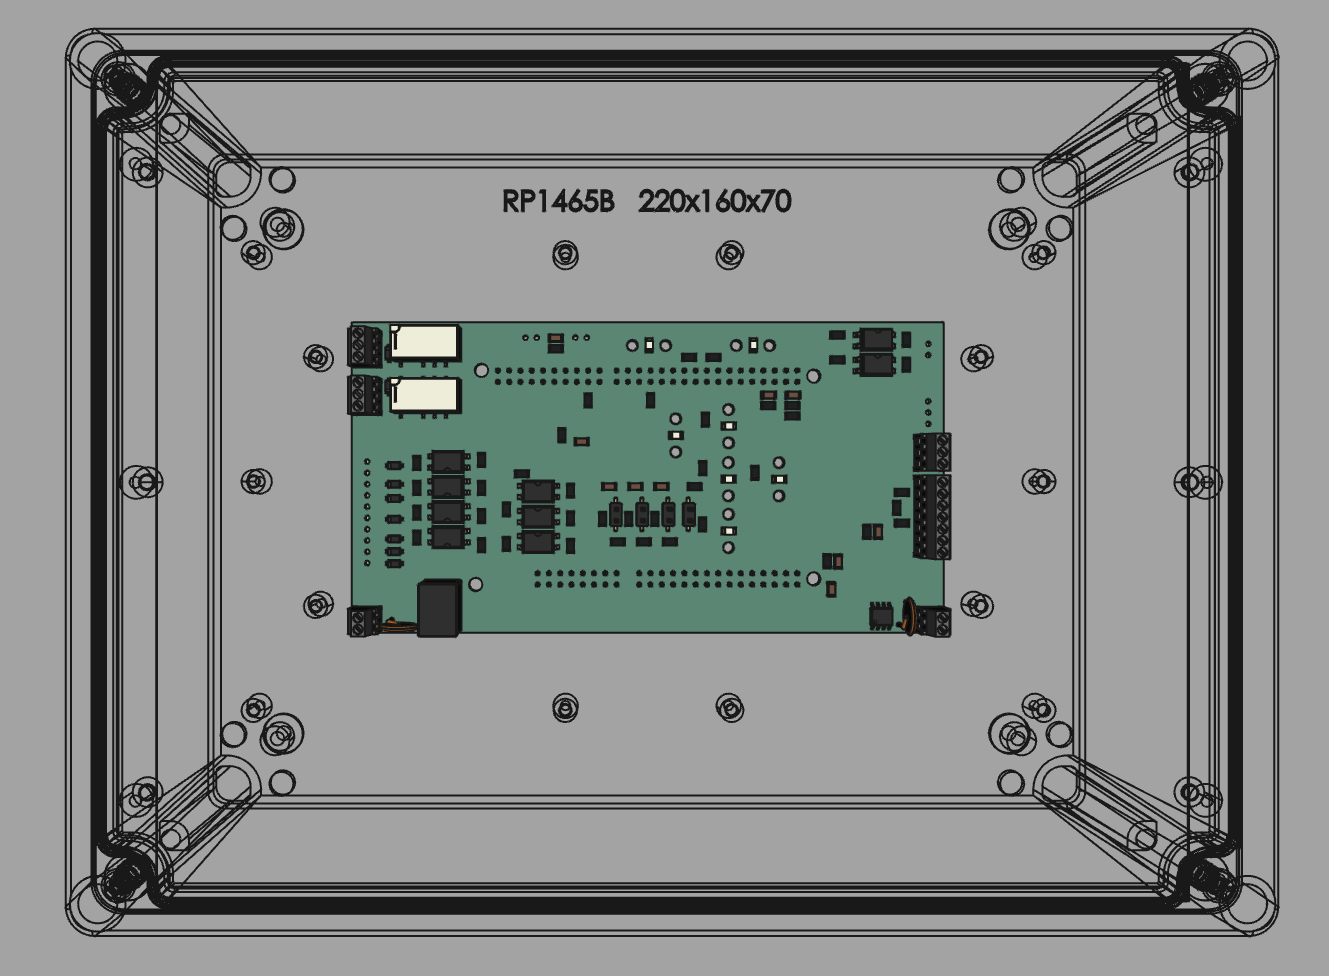
\includegraphics[width=0.8\textwidth]{images/Hardware/Platine_in_gehause.PNG}
	\caption{3D Modell der Platine innerhalb des Gehäuses}
	\label{fig:Gehaues_und_Platine}
\end{figure}
\noindent Wie in \autoref{fig:Gehaues_und_Platine} zusehen ist, bietet dieses genügend Platz für die Platine und alle Kabeldurchführungen. Es ermöglicht ebenfalls den Einsatz eines zweiten Bodens auf dem die Platine mit einer 3D gedruckten Befestigung angeschraubt werden können.\\

\subsubsection{Bedienoberfläche}
\noindent Die Bedienoberfläche besteht aus einer Reihe von Kippschaltern, Knöpfen und LEDs. Diese sind in \autoref{fig:Bedienung} dargestellt. Mit dem rechten Knopf soll zur Initialisierung des Systems eine automatische Kalibrierungsfahrt eingeleitet werden. Zusätzlich kann der Benutzer anschließend über die Trimm- und Rollknöpfe die Grenze zwischen diesen Bereichen (siehe \autoref{fig:powerCurve}) selbst anfahren und mit erneuter Betätigung des rechten Knopfes festlegen bzw. speichern. Danach kann mittels des Kippschalters in den Automatikbetrieb gewechselt werden, in dem die Steuerung vom Controllino übernommen und das Betätigen der Knöpfe folglich ignoriert wird.
Eine Reihe von LEDs gibt Feedback über den aktuellen Zustand der Linearführung. Dabei wird konstant der aktuelle Betriebsmodus durch zwei LEDs angegeben. Ebenfalls wird die Position relativ zur festgelegten neutralen Position durch zwei gelbe LEDs angegeben. Vom System selbst identifizierte Störungen werden durch eine rote LED signalisiert.\\
Die Knöpfe und Kippschalter sind jeweils mit Dichtungsringen spritzwassergeschützt am Gehäuse montiert. Die Kabel werden über Dupont-Stecker an der Platine angeschlossen. Im Gegensatz dazu sind die LEDs direkt auf der Platine platziert, wobei deren Strahlung durch flexible Lichtleiter zur Außenseite des Gehäuses geführt werden.
\begin{figure}[H]
	\centering
	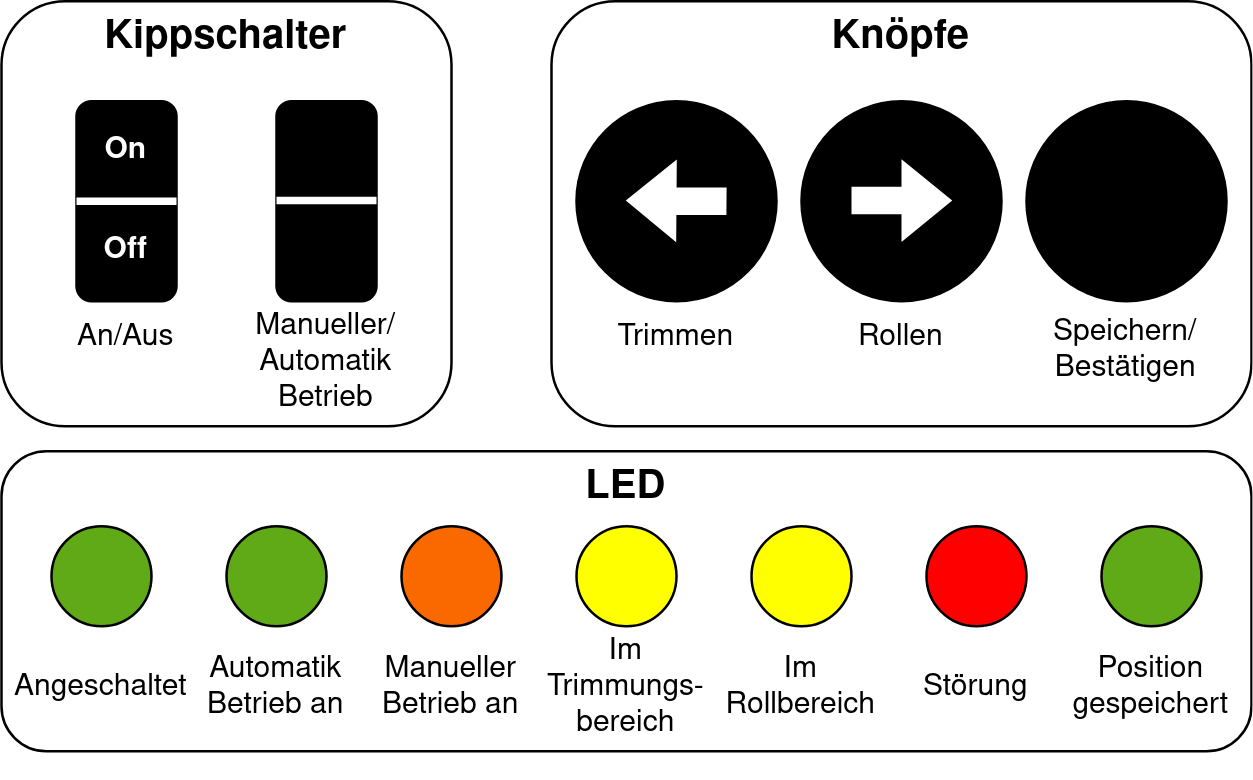
\includegraphics[width=1.0\textwidth]{images/Hardware/Bedienung.drawio.png}
	\caption{HMI der Segel Steuerung}
	\label{fig:Bedienung}
\end{figure}
\subsubsection{Kabelverschaubungen}
Um die benötigten Kabel zur Platine zuführen, wurden Kabelverschraubungen in die Seiten des Gehäuses eingelassen. In diese können die isolierten Kabel eingeführt und die Adernkabel an die richtige Position innerhalb des Gehäuses verlegt werden. Die Kabelverschraubungen sorgen nebenbei für eine Zugentlastung der Kabel.
\subsection{Platinen Schaltplan}
\begin{figure}[H]
	\centering
	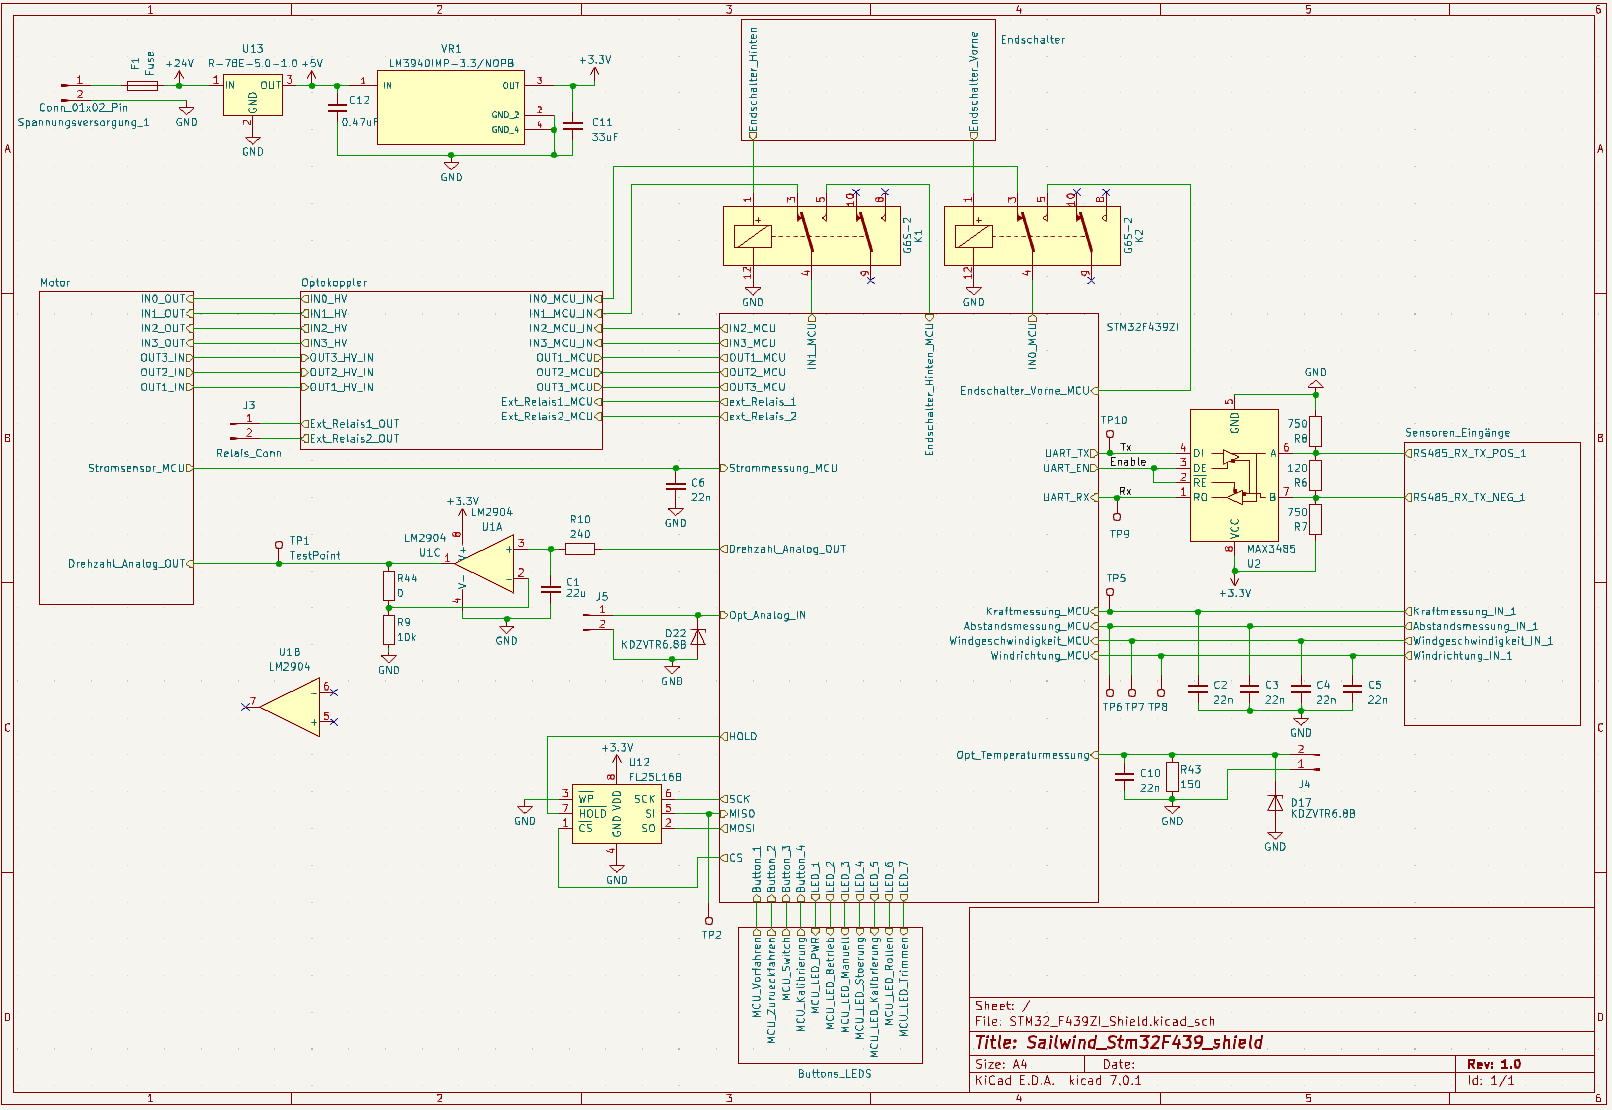
\includegraphics[width=1.0\textwidth]{images/Hardware/Schaltplan_Gesamt.PNG}
	\caption{Gesamtschaltplan der Platine}
	\label{fig:Schaltplan_gesamt}
\end{figure}
Eine Übersicht des Schaltplans ist in \autoref{fig:Schaltplan_gesamt} zusehen. Der komplette Schaltplan ist als KiCad Datei in der ZIP-Datei enthalten und ebenfalls in \autoref{sec:Schaltplan} hinterlegt. Der Schaltplan ist in unterschiedliche Bereiche eingeteilt welche die Gruppierung der Komponenten wiedergeben. Dabei ist die STM32-Gruppe zentral positioniert und alle Bauteile und Komponenten um diese herum verteilt. Bauteile, die nur einfach verbaut sind wie z.B der FL25L16B \ac{FRAM} (Unten Links) wurden nicht in Gruppen eingeteilt, sondern direkt in der Gesamtansicht positioniert. Oben links befindet sich die Spannungsversorgung der Platine und die \ac{DC}/DC Wandler. Oberhalb des STM32 befinden sich die beiden Relais, welche mit den Endschaltern verbunden sind. Links außen befindet sich der \ac{BLDC} Motor, welcher mit dem Operationsverstärker und den Optokopplern verbunden ist. Rechts befinden sich mit Ausnahme des Stromsensors alle analogen Sensoren. Dort ist ebenfalls der MAX3485 \ac{UART} Konvertierer abgebildet. Unterhalb des Mikrocontrollers befinden sich die Knöpfe und LEDS, die das \ac{HMI} bilden. Im folgenden werden exemplarisch die Schaltungen für diese Gruppen genauer betrachtet.
\subsubsection{STM32F439zi Gruppe}
Der STM32F439zi enthält alle Pins, auf denen später die Erweiterungsplatine aufsitzt. Hier wurden alle benötigten Pins nach außen zur Schaltplanübersicht geführt.
\subsubsection{Motor Gruppe}
\begin{figure}[H]
	\centering
	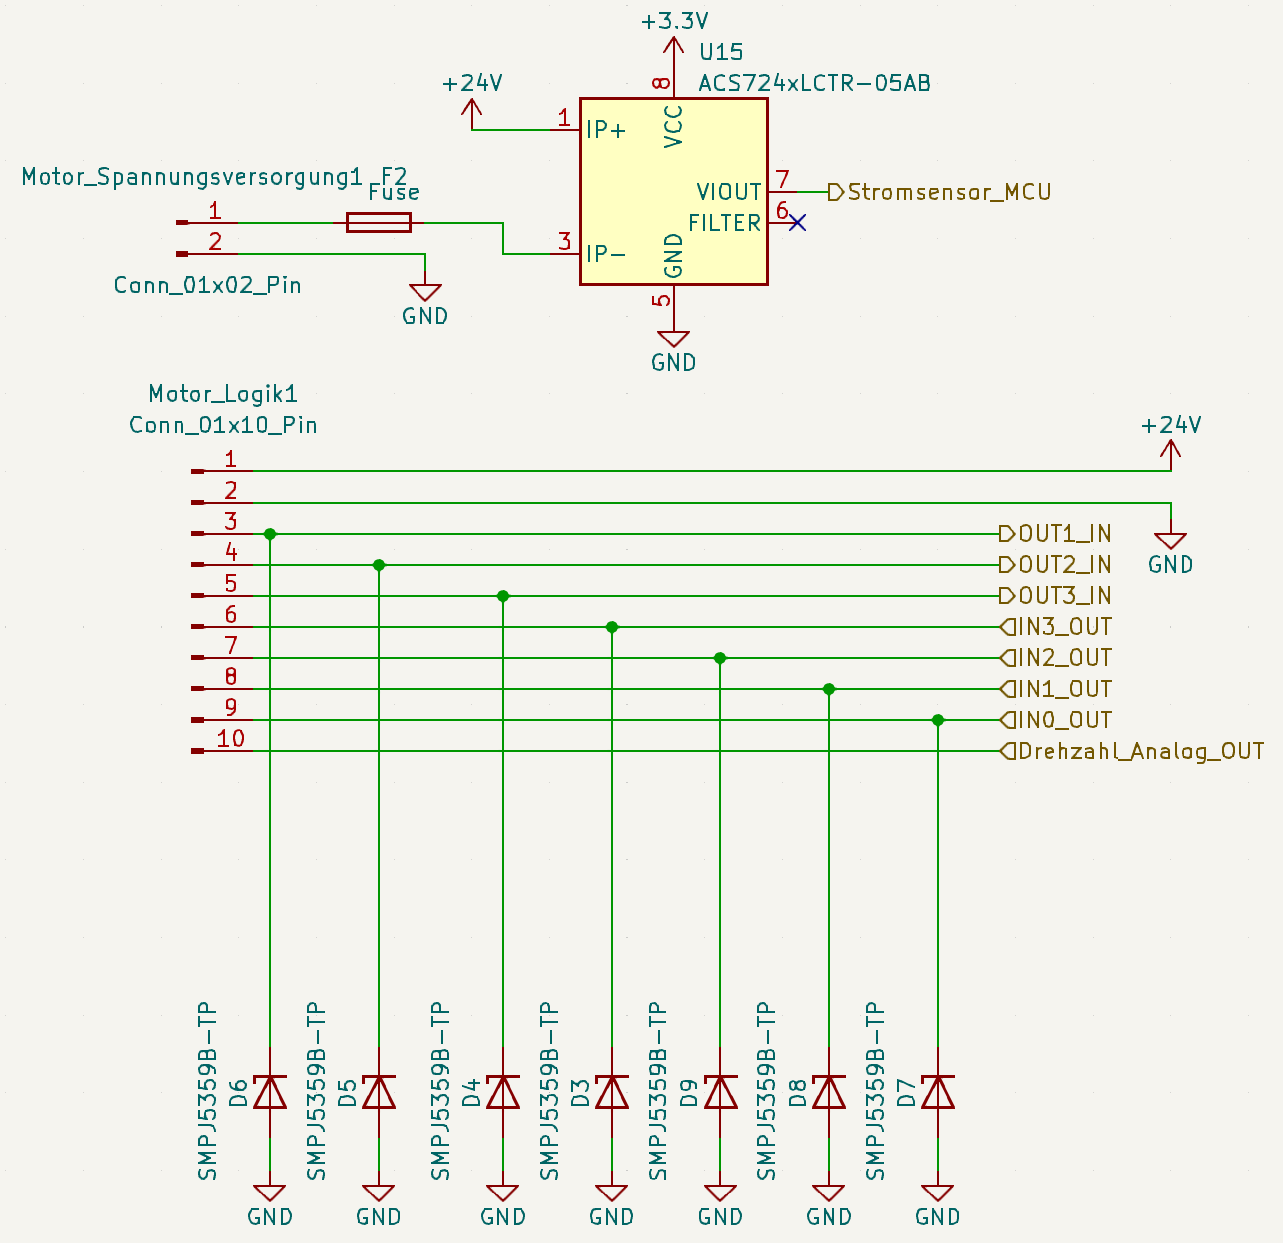
\includegraphics[width=1.0\textwidth]{images/Hardware/Motor_Schaltplan.PNG}
	\caption{Schaltplan der Motorgruppe}
	\label{fig:Motor_gruppe}
\end{figure}
In der Motorgruppe ist neben den Ein- und Ausgängen des BG 45x30 SI auch der Hall-Stromsensor abgebildet. Alle digitalen Ein- und Ausgänge auch außerhalb der Motorgruppe sind durch 24V Zener Dioden verschaltet, die als Überspannungsschutz agieren. Die Spannungsversorgungen der Platine und des Motors sind zusätzlich durch Überstromsicherungen geschützt, wie anhand des Stromsensors in \autoref{fig:Motor_gruppe} zu sehen ist.
\subsubsection{Optokoppler Gruppe}
\begin{figure}[H]
	\centering
	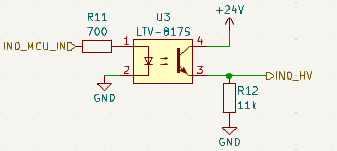
\includegraphics[width=1.0\textwidth]{images/Hardware/Optokoppler_BSP.PNG}
	\caption{Beispielhafte Schaltung eines Optokopplers}
	\label{fig:Optokoppler_gruppe}
\end{figure}
Alle Optokopplerschaltungen der Gruppe sind gleich aufgebaut. Eine beispielhafte Schaltung ist deswegen in \autoref{fig:Optokoppler_gruppe} dargestellt. Der Eingangswiderstand (links) begrenzt den Strom, welcher in der verbauten Infrarot-LED des Optokopplers den Stromfluss auf der Ausgangsseite bestimmt. Ein Pulldown-Widerstand auf der Ausgangsseite begrenzt den maximal erlaubten Strom zum Mikrocontroller und setzt den Eingang auf ein festgelegtes Potenzial.
\subsubsection{Sensoren Gruppe}
In der Sensoren Gruppe sind die analogen Sensoren abgebildet. Hier ist wie beispielhaft für den Abstandssensor in \autoref{fig:Eingang_bsp} gut zu erkennen, wie die Stromsignale in Spannungssignale von einem Widerstand umgewandelt werden. Für die 4-20mA Signale wurde dabei ein 150$\Omega$ Widerstand gewählt, da damit bei einem maximalen Strom von 20mA annähernd 3,3V erreicht werden:
\begin{equation}
	U = 20mA\times150\Omega = 3V
\end{equation}
Zum Überspannungsschutz ist hier ebenfalls eine Zener Diode mit einer Durchbruchspannung von 6,8V angebracht.
Das Spannungssignal von dem Druckkraftsensor wird durch einen Spannungsteiler ebenfalls auf 0-3V skaliert:
\begin{equation}
	U_{Ausgang} = \frac{10V}{2300\Omega + 1000\Omega}\times1000\Omega = 3,03V
\end{equation}
Um die analogen Signale stabiler zu halten und niedrige Frequenzen zu entfernen, wurden für jedes analoge Signal zusätzlich Keramikpufferkondensatoren mit einer Kapazität von 22nF hinzugefügt.
\begin{figure}[H]
	\centering
	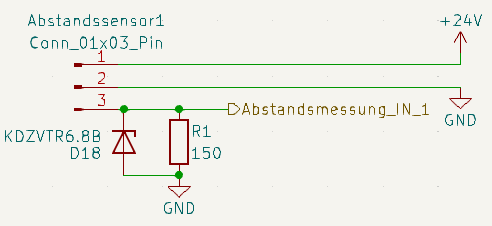
\includegraphics[width=1.0\textwidth]{images/Hardware/Analoger_Eingang.PNG}
		\caption{Schaltplan des analogen Eingangs des Abstandsensors}
	\label{fig:Eingang_bsp}
\end{figure}
\subsubsection{Buttons und LEDs Gruppe}
Damit der Effekt des Debouncing nicht über die Software ausgeregelt werden muss, wurde für die Buttons eine entsprechende Schaltung integriert. Hierbei wurde ein RC-Filter, wie in \autoref{fig:RC_Filter_Knopf} zusehen, genutzt. Beim Drücken des Knopfes wird der Kondensator zuerst entladen, was zu einer langsam abfallend Spannung führt. Wird der Knopf losgelassen, lädt sich dieser wieder auf. Somit werden jegliche unerwünschte Spannungssprünge vollständig unterdrückt. Da die Debounce-Zeit der Knöpfe typischerweise bei 0,1ms liegt (vgl. \cite{Schurter_Knopf}, S.2), wurde eine Zeitkonstante $\tau$ = 10ms für den RC Filter angenommen. Die \ac{LED}s wurden je nach zulässigem Strom mit einem entsprechenden Widerstand versehen.
\begin{figure}[H]
	\centering
	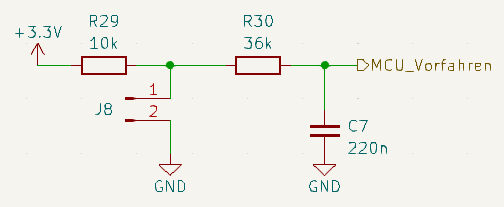
\includegraphics[width=1.0\textwidth]{images/Hardware/RC_Filter_Knopf.PNG}
	\caption{RC-Filter für einen am Gehäuse angebrachten Knopf}
	\label{fig:RC_Filter_Knopf}
\end{figure}
\subsection{\ac{PCB}}
Das fertige PCB ist als 3D Modell in \autoref{fig:PCB_3D} dargestellt. Beim Entwurf wurde darauf geachtet, die 24V- von den 3,3V-Komponenten zu trennen, um die Beeinflussung analoger Signale durch große Ströme oder höhere Frequenzen so weit wie möglich zu reduzieren. Aus diesem Grund befinden sich die 24V-Komponenten am Rand der Platine, während die 3,3V-Bauteile weitestgehend im Inneren der Platine positioniert sind. Die Platine sitzt mit vier unterschiedlichen Pin-Reihen am Entwicklungsboard auf und führt diese auf die Oberseite. Die Spurbreiten auf der Platine wurden aufgrund von Stromflüssen, Spannungen und Längen bestimmt. Da der Platinenhersteller eine minimale Spurbreite von 0,2mm vorgibt, reichte diese für fast alle Spuren aus. Eine Ausnahme bildet jene, welche dem Motorstrom von bis zu 4A ausgesetzt ist und dementsprechend breiter ausgelegt werden musste. 
\begin{figure}[H]
	\centering
	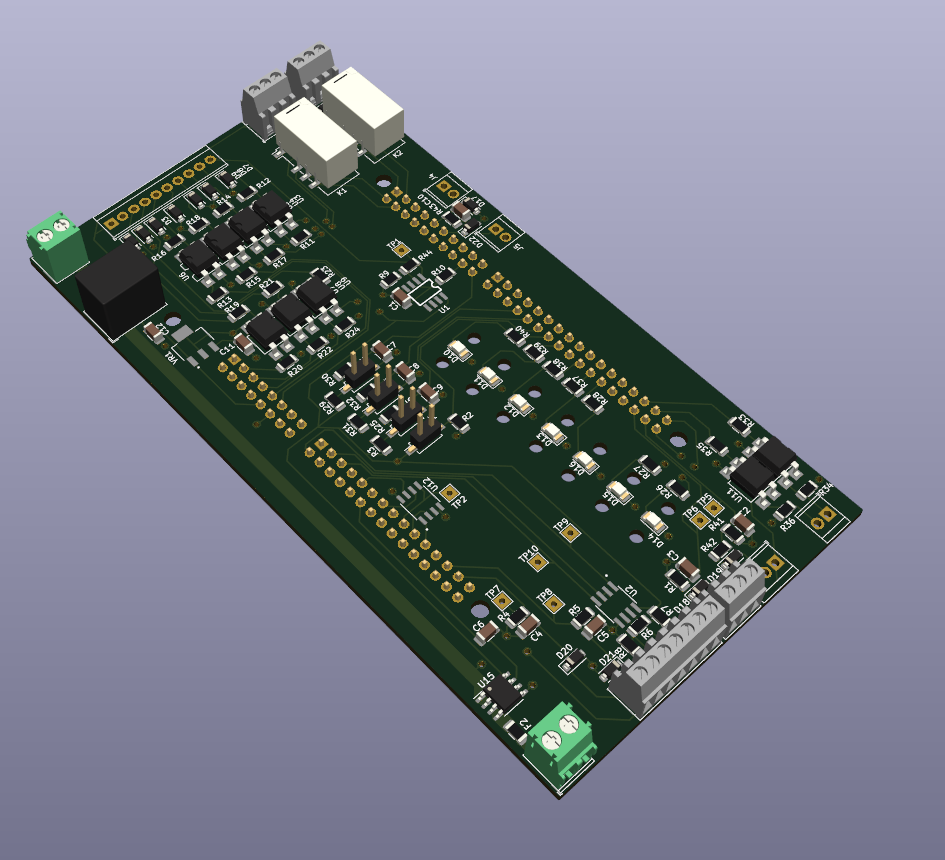
\includegraphics[width=1.0\textwidth]{images/Hardware/Platine_Fertig_3D_ansicht(1).PNG}
	\caption{3D Ansicht des fertigen PCBs}
	\label{fig:PCB_3D}
\end{figure}
Der Formfaktor der Platine wurde an dem Standard Layout eines ST Nucleo 144 Boards orientiert. Aufgrund des damit verfügbaren Platzes wurden ausschließlich \ac{SMD} Bauteile der Größe 1206 verwendet. Diese sind groß genug, um sie unter angemessenem Aufwand von Hand zu löten und andererseits klein genug, um geeignete Abstände bei der Positionierung einhalten zu können. Eine Liste aller verwendeter Platinen- und Gehäusebauteile ist in \autoref{sec:Bauteilliste} zu finden.

\subsection{Probleme}
Während der Nutzung und Bestückung des \ac{PCB}s sind einige Probleme aufgetreten, die auf das Design oder falsche Berechnungen zurückzuführen sind. Diese sollen im folgenden erklärt und korrigiert werden.
\subsubsection{Schraubklemmen Löcher}
Der erste Fehler, welcher zu Beginn auffiel, waren die Lochdurchmesser für die Schraubklemmen. Diese waren zwar groß genug dimensioniert, um die Pins der Schraubklemmen durchzuführen, jedoch fehlte damit der Platz, um Nieten zur elektrischen Verbindung zwischen den Pins und der Platine einzufügen. Die Löcher waren ebenfalls zu klein, um mit Drähten eine Verbindung zwischen dem Pin und den Spuren herzustellen. Dies führte zu vielen elektrischen Kontaktverlusten und minderte die horizontale Stabilität der Schraubklemmen. Die Kontaktverluste führten wiederum zur mangelnden Präzision der analogen Eingänge (siehe \autoref{Mangelnde_Präzision}). Da die Löcher im Nachhinein nicht mehr vergrößert werden konnten, gab es hierfür leider keine Möglichkeit, diesen Fehler auszubessern.
\subsubsection{Operationsverstärker}
Der Operationsverstärker war zwar als Verstärkerschaltung richtig konfiguriert, allerdings musste die Verstärkerspannung von 3,3V auf 24V angehoben werden, um die 10V zu erreichen. Zusätzlich wurde der Spannungsteiler am Ausgang des OPVs entfernt und der erste Widerstand gegen einen Jumper getauscht.
\subsubsection{RS485 Bias Widerstände}
Die RS485 Widerstände wurden anfänglich nach den empfohlenen Werten in der WSWD Dokumentation dimensioniert. Hier wurde bei einer Versorgungsspannung von 5V ein Busabschlusswiderstand $R_t$ von 120$\Omega$ und zwei Bias-Widerstände $R_b$ von 750$\Omega$ empfohlen (vgl.\cite{WSWD} S.21). Dies sorgte allerdings für eine zu große Differenz der beiden Spannungen und der MAX3485 konnte nicht zwischen HIGH und LOW unterscheiden. Deshalb wurde stattdessen nach der Anleitung des MAX3485 die Differenz zwischen beiden Potenzialen auf 0,2V begrenzt. Hierfür wurde auf die Berechnung in dem von Texas Instruments veröffentlichten Bericht: \glqq{}RS-485 failsafe for an idle bus\grqq{} zurückgegriffen (vgl. \cite{Texas_instruments}). Mithilfe der Formel: 
\begin{equation}
	R_b = (\frac{V_s}{V_{diff }}+1)\times27,8\Omega
\end{equation}
lassen sich die beiden Bias Widerstände für das RS-485 Netzwerk berechnen. Aus den eingesetzten Werten resultiert:
\begin{equation}
	R_b = (\frac{3,3V}{0,2V}+1)\times27,8\Omega = 486,5\Omega
\end{equation}
Der nächstkleinere Widerstand der verfügbaren E24-Reihe wurde mit 470$\Omega$ gewählt. Damit konnte schließlich erfolgreich über RS485 kommuniziert werden.
\subsubsection{FRAM Anschlüsse}
Die SPI-Anschlüsse des FRAM Speichers wurden falsch verbunden. Dabei wurden die \ac{MOSI}- und \ac{MISO}-Leitung vertauscht und der \ac{WP}-Pin auf das Ground-Potenzial gelegt. Dies führte dazu, dass der Speicher nicht adressiert werden konnte und folglich nicht auf gesendete Befehle reagierte. Zuerst wurde der \ac{WP} von dem Ground Potenzial entfernt und schwebend gehalten. Durch das Beobachten der Pegel von MISO-, MOSI- und Clock-Leitung konnte daraufhin erkannt werden, dass diese vertauscht wurden. Die PCB-Spur wurde dementsprechend getrennt und die Pins stattdessen mit Kabeln verbunden.
\subsubsection{Abstandssensor Präzision}
Der Abstandssensor war eine weitere, große Fehlerquelle. Der Abstandsensor hat zwar eine sehr hohe Präzision erreicht, allerdings erst nach einer Aufwärmzeit. Dieser Effekt tritt laut Datenblatt erst unter einer Umgebungstemperatur von -10°C auf (vgl. \cite{OGD580_Datasheet} S.2). Jedoch wurde in mehreren Tests festgestellt, dass bei Stillstand das Display des Sensors mit der Zeit sinkende Werte anzeigt. Um die Ursache dafür zu finden, wurden einige Messreihen durchgeführt. Hierbei wurde der Abstand zum Sensor konstant gehalten und in einem Intervall von 30s der Spannungswert an einem Messpunkt der Platine mit einem Oszilloskop gemessen. Dies wurde für inkrementierende Außerbetriebszeiten wiederholt. Die Messreihe ist in \autoref{fig:Messreihe_Temperatur} dargestellt. Hier ist klar erkennbar, dass erst nach ca. 1400s bzw. 20-25min ein gleichbleibender Spannungswert auslesbar ist. Ebenfalls geht daraus hervor, dass die Präzision mit der Temperatur des Sensors zusammenhängt, da nach kürzeren Außerbetriebszeiten die Differenz sinkt.
\begin{figure}[H]
	\centering
	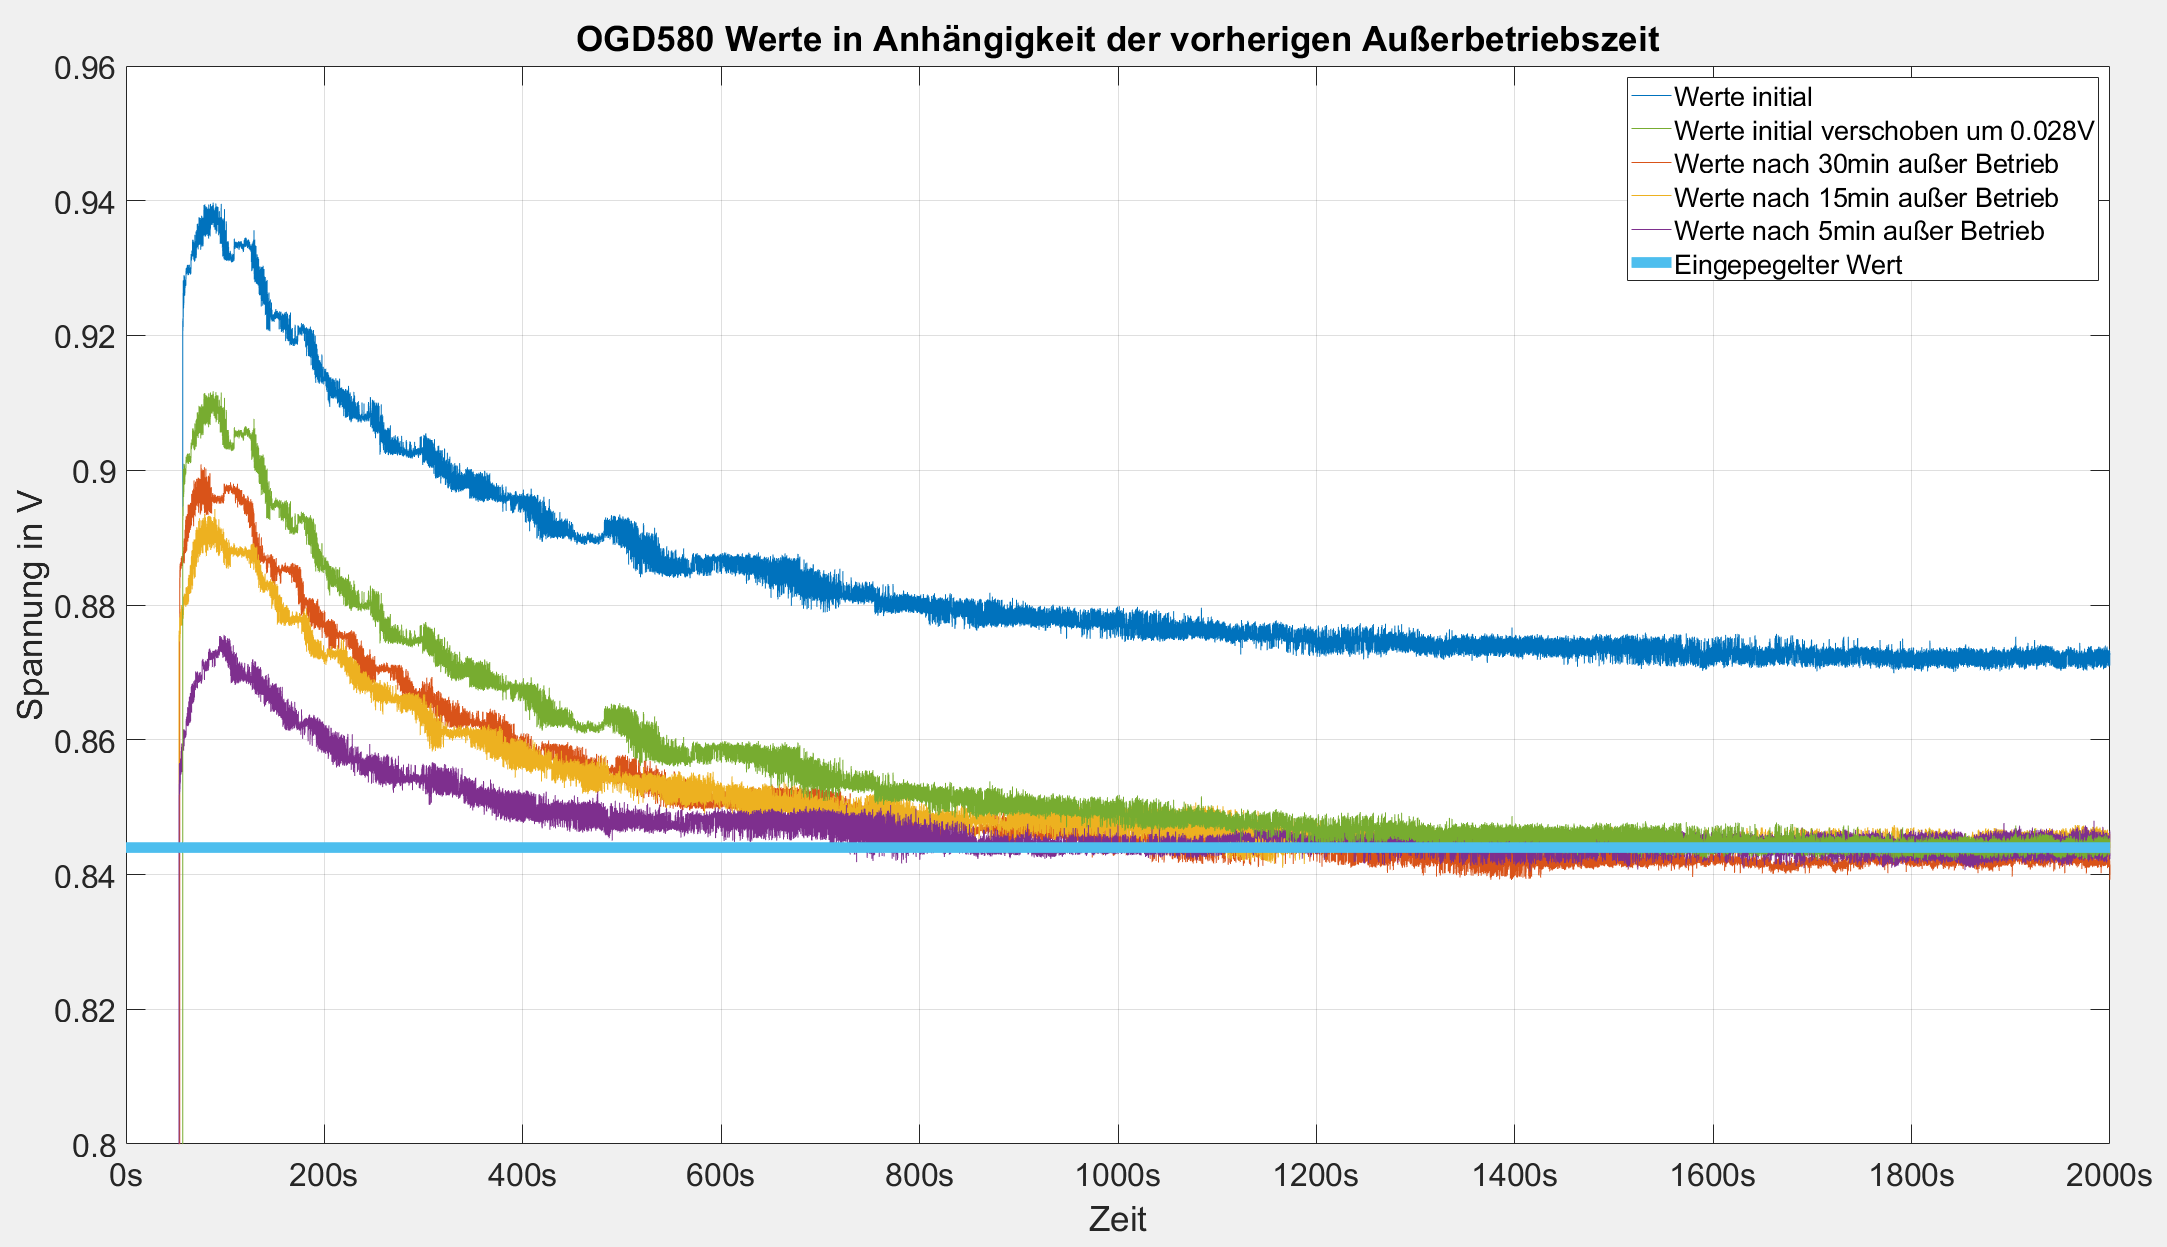
\includegraphics[width=1.0\textwidth]{images/Hardware/Abstandssensor_plot_highres.PNG}
	\caption{Messreihen des ausgelesen Spannungswert bei gleichbleibendem Abstand und steigenden Außerbetriebszeiten}
	\label{fig:Messreihe_Temperatur}
\end{figure}

Das Problem blieb allerdings selbst nach einer Aufwärmzeit von 20min. bestehen. Die Abweichungen der ausgelesenen Werte über die Messpunkte von den Werten am Display lagen teilweise bei 25mm. Um die Ursache dieses Problems zu finden, wurden weitere Messreihen aufgenommen. Dabei wurde der Schlitten der Linearführung in 20mm Abständen verschoben. An jedem dieser Punkte wurden folgende Daten notiert:
\begin{itemize}
	\item Abstand zum Sensor, gemessen mit einem Meterstab in mm
	\item Angezeigter Abstand auf dem Display des Sensors in mm
	\item Ausgegebener Strom des IO-Link Konverters gemessen mit einem Multimeter in mA
	\item Spannung am Testpunkt der Platine mit einem Oszilloskop in V
\end{itemize}
Dies wurde in 5 Messreihen wiederholt, um die Reproduzierbarkeit zu verifizieren. Die aufgezeichneten Daten wurden in mm umgerechnet:
\begin{equation}
	L_{Strom} = \frac{L_{max}-L_{min}}{I_{max}-I_{min}}\times(\frac{I_{Position}}{1000}-I_{min}) + L_{min}
\end{equation}
\begin{equation}
	L_{Spannung} = \frac{L_{max}-L_{min}}{I_{max}-I_{min}}\times(\frac{U_{Position}}{153,5\Omega}-I_{min}) + L_{min}
\end{equation}
 und oberhalb der mit dem Meterstab gemessenen Werte geplottet. Eine dieser Messreihen ist in \autoref{fig:Messreihe_Abstand} dargestellt.
\begin{figure}[H]
	\centering
	\includegraphics[width=1.0\textwidth]{images/Hardware/Messreihe_Präzision.png}
	\caption{Präzision des Abstandssensors anhand verschiedener Messwerte}
	\label{fig:Messreihe_Abstand}
\end{figure}
\noindent Hier ist zu erkennen, dass der auf dem Display abgelesene mit dem gemessenen Abstand übereinstimmt. Allerdings weichen sowohl der Strom- als auch der Spannungswert ab, da die Steigung beider Messreihen nicht gleich zu der des Abstandssensors ist. Dieser ermöglicht die Anpassung der Skalierung. Dabei kann z.B festgelegt werden, ab welchem Messwert das Ausgangssignal 4mA/20mA betragen soll (vgl. \cite{EIO104_Manual}, S.6). Da das Display den korrekten Wert anzeigt, aber ein falscher Strom Wert ausgegeben wird, kann davon ausgegangen werden, dass der Konverter falsch eingestellt ist. Dies konnte im Zuge dieser Arbeit nicht behoben werden, da ein entsprechendes IO-Link Master Gerät nicht verfügbar war.
\subsubsection{Präzision der Analogen Signale}
\label{Mangelnde_Präzision}
Neben den Problemen mit dem Abstandssensor wurden ebenfalls leicht abweichende Werte in den anderen Analogsignalen festgestellt. Beginnend mit den Stromsignalen, kann der ausgelesene Wert mit der Präzision des Widerstandes zusammenhängen, da diese mit 1\% Genauigkeit immer noch große Temperaturabweichungen aufweisen können. Die schlechten Kontakte tragen ebenfalls zur Ungenauigkeit bei. Speziell beim Stromsensor kann auch hier die Positionierung eine Fehlerquelle sein, da die verbundenen Spuren für optimale Präzision im 45° Winkel zu den Sensorpins stehen sollten. Um die Präzision zu verbessern, können zusätzlich zu den Widerständen Ferrite eingesetzt werden. Diese verhalten sich ähnlich wie Spulen und filtern hochfrequente Signale. In Kombination mit den bereits verwendeten Kondensatoren würden diese einen LC-Filter darstellen und einen Bandpass erzeugen, der zusätzlich die Signalqualität verbessert.\\
